\title{Solutions for Homework 2}
\author{Dr. Jordan Hanson - Whittier College Dept. of Physics and Astronomy}
\date{\today}
\documentclass[10pt]{article}
\usepackage[a4paper, total={18cm, 27cm}]{geometry}
\usepackage{graphicx}
\usepackage{amsmath}
\usepackage{tcolorbox}

\def\rcurs{{\mbox{$\resizebox{.16in}{.08in}{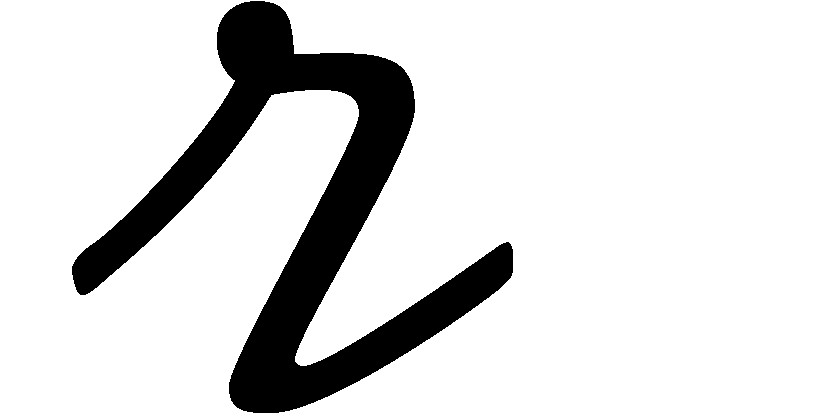
\includegraphics{ScriptR}}$}}}
\def\brcurs{{\mbox{$\resizebox{.16in}{.08in}{
\includegraphics{BoldR}}$}}}
\def\hrcurs{{\mbox{$\hat \rcurs$}}}

\begin{document}
\maketitle

\section{Problem 2.5}

\textit{Find the electric field a distance $z$ above the center of a circular loop of radius $r$ that carries a uniform line charge $\lambda$.} \\ \\

Start by filling in the pieces of the Coulomb effect:

\begin{equation}
d\mathbf{E} = \frac{1}{4\pi\epsilon_0}\frac{dq'}{\rcurs^2}\hrcurs
\end{equation}

\begin{itemize}
\item $\brcurs = z \hat{z} - R\hat{s}$
\item $\rcurs = \sqrt{z^2 + R^2} = z\sqrt{1+(R/z)^2} = z\sqrt{1+\epsilon^2}$. (If $\epsilon \to 0$, this represents the far-field).
\item $\rcurs^2 = z^2 + R^2$
\item $\hrcurs = (\hat{z} - \epsilon \hat{s})/(1+\epsilon^2)^{1/2}$
\item $dq' = \lambda R d\phi'$, because cylindrical coordinates are the correct choice here.
\item Note that $\epsilon = R/z$, so if $z = 0$ then $\epsilon \to \infty$, and $\epsilon \to 0$ if $z \gg R$.
\item $Q = 2\pi R\lambda$, the total charge.
\end{itemize}

Integrate to add up the $d\mathbf{E}$ to find $\mathbf{E}$:

\begin{equation}
\mathbf{E} = \frac{\lambda R}{4\pi\epsilon_0 z^2 (1+\epsilon^2)^{3/2}} \int_0^{2\pi} d\phi' (\hat{z} - \epsilon \hat{s})
\end{equation}

By symmetry, the $\hat{s}$ term evaluates to zero.  The result is

\begin{equation}
\mathbf{E} = \frac{2\pi\lambda R \hat{z}}{4\pi\epsilon_0 z^2 (1+\epsilon^2)^{3/2}} = \frac{Q\hat{z}}{4\pi\epsilon_0 z^2 (1+\epsilon^2)^{3/2}}
\end{equation}

Checks: $\mathbf{E} = 0$ if $z = 0$ because $\epsilon \to \infty$.  Also, we find the far-field effect if $z \ll R$, because $\epsilon \to 0$.  The units also check out.

\section{Problem 2.6}

\textit{Find the electric field a distance $z$ above a the center of a flat circular disc of radius $R$ that carries a uniform surface charge $\sigma$.  What does your formula give in the limit $R \to \infty$? Also check the case $z \gg R$.} \\ \\

Start by filling in the pieces of the Coulomb effect:

\begin{equation}
d\mathbf{E} = \frac{1}{4\pi\epsilon_0}\frac{dq'}{\rcurs^2}\hrcurs
\end{equation}

\begin{itemize}
\item $\brcurs = z\hat{z} - s\hat{s}$.  As in Problem 2.5, the $\hat{s}$-component will vanish upon integration.
\item $\rcurs^2 = z^2 + s^2$
\item $\hrcurs = (z\hat{z} - s\hat{s})/(z^2 + s^2)^{1/2}$
\item $dq' = \sigma da' = s ds d\phi$, because cylindrical coordinates work best here.
\item $Q = \pi R^2 \sigma$ is the total charge.
\item Let $z\tan\theta = s$, so that $ds = z\sec^2\theta d\theta$, and $\theta_0 = \tan^{-1}(R/z)$
\end{itemize}

Integrate to add up the $d\mathbf{E}$ to find $\mathbf{E}$:

\begin{align}
\mathbf{E} &= \frac{\sigma}{2\epsilon_0} z \hat{z} \int_0^R \frac{s ds}{(s^2+z^2)^{3/2}} \\
\mathbf{E} &= \frac{\sigma}{2\epsilon_0} \left.\cos\theta \right\vert_0^{\theta_0} \hat{z} = \frac{\sigma}{2\epsilon_0} \left( 1 - \cos\theta_0 \right) \hat{z}
\end{align}

We know what is $\tan\theta = R/z$, but what is $\cos\theta_0$?  (\textit{Hint: draw the triangle and then find the hypoteneuse}).  The result is

\begin{equation}
\mathbf{E} = \frac{\sigma \hat{z}}{2\epsilon_0}\left( 1 - \frac{z}{\sqrt{z^2 + R^2}}\right)
\end{equation}

The units check automatically because of the units of $\sigma$ (Coulombs per meter squared), and the $\epsilon_0$ in the denominator.  If $R \to \infty$, then the second term vanishes and the field is 

\begin{equation}
\mathbf{E} \to \frac{\sigma \hat{z}}{2\epsilon_0}
\end{equation}

This form of the field is the boundary condition near a charged surface.  To check the limit that $z \gg R$, first factor a $z$:

\begin{equation}
\mathbf{E} = \frac{\sigma \hat{z}}{2\epsilon_0} z \left( z^{-1} - (z^2 + R^2)^{-1/2}\right) = \frac{\sigma \hat{z}}{2\epsilon_0} z \left( z^{-1} - z^{-1} (1 + (R/z)^2)^{-1/2}\right)
\end{equation}

Now replace $(1+(R/z)^2)^{-1/2} \approx (1 - (1/2) (R/z)^2)$, and notice the $1/z$ terms cancel:

\begin{equation}
\mathbf{E} = \frac{\sigma \hat{z}}{2\epsilon_0}z\left( \frac{1}{2z} \left(\frac{R}{z}\right)^2 \right)
\end{equation}

Multiply top and bottom by $\pi$, and recall that $Q = \pi R^2$ to find the point-charge field:

\begin{equation}
\mathbf{E} = \frac{1}{4\pi\epsilon_0} \frac{Q \hat{z}}{z^2}
\end{equation}

\section{Problem 2.9}

\textit{Suppose the electric field in some region is found to be $\mathbf{E} = k r^3 \hat{r}$, in spherical coordinates (k is some constant). (a) Find the charge densiy $\rho$. (b) Find the total charge contained in a sphere of radius $R$, centered at the origin. (Do it two ways).} \\ \\

(a) This is a straightforward application of Gauss' Law in differential form, noting that only the $\hat{r}$ term matters by symmetry:

\begin{equation}
\nabla \cdot \mathbf{E} = \frac{1}{r^2} \frac{\partial}{\partial r}\left( r^2 \mathbf{E} \cdot \hat{r} \right) + ... = 5kr^2
\end{equation} 

Thus the charge distribution is 

\begin{equation}
\rho(r) = 5 k \epsilon_0 r^2 \label{eq:rho}
\end{equation}

(b) The total charge $Q$ may be found by (i) direct integration of Eq. \ref{eq:rho}, or (ii) by using Gauss' Law.  First, (i):

\begin{equation}
Q = \int \rho(r) d\tau = \int_0^{R} \int_0^{\pi} \int_0^{2\pi} 5 k \epsilon_0 r^2 r^2 \sin\theta dr d\theta d\phi = (4\pi)(5k\epsilon_0) \int_0^{R} r^4 dr = 4\pi k \epsilon_0 R^5
\end{equation}

Now, method (ii): 

\begin{equation}
Q = \epsilon_0 \oint \mathbf{E} \cdot d\mathbf{a} = \epsilon_0 \int_0^{2\pi} \int_0^{\pi} k R^3 \hat{r} \cdot \hat{r} R^2 d\theta d\phi = 4\pi k \epsilon_0 R^5
\end{equation}

\section{Problem 2.12}

\textit{Use Gauss' Law to find the electric field inside a uniformly charged solid sphere (charge density $\rho$).} \\ \\

Note that

\begin{itemize}
\item $d\mathbf{a} \propto \hat{r}$
\item $\mathbf{E} \propto \hat{r}$ and only varies with $r$, by symmetry.
\item Along a spherical Gaussian surface at radius $r$, $\mathbf{E}$ is constant.
\item Thus, $\oint \mathbf{E} \cdot d\mathbf{a} = \mathbf{E} \cdot \mathbf{A}$, where $\mathbf{A}$ is the surface area of the Gaussian surface oriented in the $\hat{r}$ direction.
\end{itemize}

We now have

\begin{equation}
\mathbf{E} \cdot \mathbf{A} = \frac{1}{\epsilon_0} \rho \int d\tau' = \frac{\rho}{\epsilon_0} (4\pi) \int_0^{r} r'^2 dr'
\end{equation}

The final result is

\begin{equation}
\mathbf{E}(\mathbf{r}) = \frac{\rho \mathbf{r}}{3\epsilon_0} = \frac{\rho r\hat{r}}{3\epsilon_0}
\end{equation}

\section{Problem 2.16}

\textit{A long coaxial cable carries a uniform volume charge density $\rho$ on the inner cylinder (radius a), and a uniform surface charge density on the outer cylindrical shell (radius b). This surface charge is negative and is of just the right magnitude that the cable as a whole is electrically neutral.  Find the electric field in each of the three regions: (i) inside the inner cylinder $(s < a)$, (ii) between the cylinders $(a < s < b)$, (iii) outside the cable $(s > b)$.  Plot $|\mathbf{E}|$ as a function of $s$.}

\begin{itemize}
\item $(s < a)$: By symmetry, $\mathbf{E} \propto \hat{s}$, and we simplify Gauss' Law to read 
\begin{align}
\mathbf{E} \cdot \mathbf{A} &= \frac{Q}{\epsilon_0} \\
E (2\pi s) z &= \frac{1}{\epsilon_0}\int \rho' d\tau' \\
E (2\pi s) z &= \frac{1}{\epsilon_0}\int_0^s \rho s'ds' (2\pi) z \\
\mathbf{E} &= \rho \frac{s\hat{s}}{2\epsilon_0}
\end{align}
\item $(a < s < b)$: By symmetry, $\mathbf{E} \propto \hat{s}$, and we simplify Gauss' Law to read
\begin{align}
\mathbf{E} \cdot \mathbf{A} &= \frac{Q}{\epsilon_0} \\
E (2\pi s) z &= \rho (\pi a^2 z)/\epsilon_0 \\
\mathbf{E} &= \frac{\rho a^2}{2 s \epsilon_0}\hat{s}
\end{align}
\item $(s > b)$: The cable is electrically neutral, so our Gaussian surface contains the same amount of positive and negative charge.  Thus:
\begin{equation}
\mathbf{E} = \mathbf{0}
\end{equation}
\end{itemize}

The graph should show that $\mathbf{E}$ is linearly increasing until $s = a$, after which it falls as $1/s$.  Outside, it drops to zero.

\section{Problem 2.18}

\textit{Two spheres, each of radius $R$ and carrying uniform volume charge densities $\rho$ and $-\rho$, respectively, are placed so that they partially overlap.  Call the vector from the positive center to the negative center $\mathbf{d}$.  Show that the field in the region of overlap is constant, and find its value.  Use the answer to Problem 2.12.} \\ \\

Suppose the observer is at a point $P$ within the overlap region, and $\mathbf{r}_{+}$ and $\mathbf{r}_{-}$ are the displacements from positive and negative sphere centers to $P$, respectively.  If $\mathbf{d}$ points from the positive center to the negative center, then

\begin{equation}
\mathbf{d} = \mathbf{r}_{+} - \mathbf{r}_{-} \label{eq:d}
\end{equation}

Using the field result from 2.12 to sum the contributions from positive and negative spheres, and Eq. \ref{eq:d}, we find

\begin{align}
\mathbf{E} &= \frac{\rho\mathbf{r}_{+}}{3\epsilon_0} - \frac{\rho\mathbf{r}_{-}}{3\epsilon_0} \\
\mathbf{E} &= \frac{\rho\mathbf{d}}{3\epsilon_0}
\end{align}

\section{Problem 2.25}

\textit{Using equations describing the potential of point, line, and surface charges, find the potential at a distance $z$ above the center of (i) a pair of positive charges separated by a distance $d$, (ii) a line charge of length $2L$, and (iii) a uniform surface charge spread into a disc of radius $R$.  Compute $\mathbf{E} = -\nabla V$ in each case, and check the results for the fields against prior results.  What is the value of the potential at the same point above the pair of charges if the right-hand one is negative?  What does that suggest about the direction of the field?  Compare this to prior results carefully.} \\ \\

Let $k = 1/(4\pi\epsilon_0)$. The situation for each distribution is summarized below.

\begin{itemize}
\item \textbf{Pair of point charges:} The displacement between each charge and $P = z$ is the same: $\rcurs = \sqrt{z^2 + \frac{1}{4}d^2}$.  Thus, the total potential is
\begin{equation}
V(z) = \frac{2kq}{\rcurs} = \frac{2 k q}{(z^2 + \frac{1}{4}d^2)^{1/2}}
\end{equation}
Compute the field by taking the negative gradient:
\begin{equation}
-\frac{dV}{dz}\hat{z} = \frac{2 k q z \hat{z}}{(z^2 + \frac{1}{2}d^2)^{3/2}}
\end{equation}
That does match our result from earlier.
\item \textbf{The line charge of length $2L$:} Let the charge density be $\lambda$.  The contribution to the potential from $dq' = \lambda dx'$ is
\begin{equation}
dV = \frac{k \lambda dx'}{(x'^2 + z^2)^{1/2}}
\end{equation}
The integral can be done via trigonometric substitution or simply looking it up in a table:
\begin{equation}
V(z) = k\lambda \ln \left(\frac{\sqrt{z^2 + L^2} + L}{\sqrt{z^2 + L^2} - L}\right)
\end{equation}
Taking the negative derivative with respect to $z$, following the chain rule inside the logarithm, and simplifying yields
\begin{equation}
\mathbf{E} = 2kL\lambda \frac{1}{z\sqrt{z^2 + L^2}}\hat{z}
\end{equation}
This agrees with prior results and checks out in the far-field limit.
\item \textbf{The disc of charge with radius $R$, with density $\sigma$:}
\begin{equation}
dV = \frac{k dq'}{\rcurs} = \frac{k \sigma da'}{\sqrt{s'^2 + z^2}} = \frac{k\sigma s'ds'd\phi'}{\sqrt{s'^2 + z^2}}
\end{equation}
Perform the integral:
\begin{equation}
V(z) = \frac{\sigma}{2\epsilon_0}\left( \sqrt{R^2+z^2} - z \right)
\end{equation}
The negative gradient shows us that
\begin{equation}
\mathbf{E} = \frac{\sigma}{2\epsilon_0}\left(1 - \frac{z}{\sqrt{z^2 + R^2}}\right)\hat{z}
\end{equation}
This agrees with our prior result for the $\mathbf{E}$-field.
\item If we swap the right-hand charge from positive to negative, then $V(z) = 0$ on the whole z-axis.  We shouldn't conclude that $\mathbf{E} = 0$ because we only know that $dV/dz = 0$.  Examining the charges again, we can sketch the field to find that it now points in the x-direction, so $dV/dx \neq 0$.
\end{itemize}

\section{Problem 2.29}

\textit{Check that the Laplacian of the volume integral that defines potential gives the charge density.  That is, show that $\nabla^2 V(\mathbf{r}) = -\rho/\epsilon_0$.} \\ \\
The electrostatic potential, in general, is
\begin{equation}
V(\mathbf{r}) = \frac{1}{4\pi\epsilon_0}\int \frac{\rho(\mathbf{r}') d\tau'}{\rcurs}
\end{equation}
The key to this argument is that the $\nabla^2$ operator acts on functions of $\mathbf{r}$, not $\mathbf{r}'$.  Thus,
\begin{equation}
\nabla^2 V(\mathbf{r}) = \frac{1}{4\pi\epsilon_0}\int \rho(\mathbf{r}') d\tau'\nabla^2 \left(\frac{1}{\rcurs}\right) \label{eq:V}
\end{equation}
\textbf{But due to our diligence on the last assignment} ... we see that
\begin{equation}
\nabla^2 \left(\frac{1}{\rcurs}\right) = -4\pi\delta^3(\mathbf{r}-\mathbf{r}')
\end{equation}
Substituting the $\delta$-function into Eq. \ref{eq:V}:
\begin{equation}
\nabla^2 V(\mathbf{r}) = -\frac{4\pi}{4\pi\epsilon_0} \int \rho(\mathbf{r}')\delta^3(\mathbf{r}-\mathbf{r}')d\tau' = \rho(\mathbf{r})/\epsilon_0
\end{equation}
\end{document}
